%Standard Dokumenten Einstellungen
%Einstellen der Schriftgröße
% \documentclass[a4paper,12pt]{scrreport}
\documentclass[a4paper,11pt, parskip=full]{scrreprt}

% Eingabe der benötigten Konfigurationen
% !TeX root = ../template.tex

%Inhalt der Titelseite
\newcommand{\Titel}{Einarbeitung in die agile Softwareentwicklung von modularen, containerisierten Software Applikationen}
\newcommand{\Art}{T3000}
\newcommand{\Vorname}{Jannis}
\newcommand{\Nachname}{Reksztat}
\newcommand{\Studiengang}{Elektrotechnik}
\newcommand{\Abgabedatum}{19.06.2023}
\newcommand{\Bearbeitungszeitraum}{03.04.2023 - 19.06.2023}
\newcommand{\Matrikelnummer}{7962000}
\newcommand{\Kurskrzl}{TEL20AT1}
\newcommand{\Ausbildungsfirma}{ABB AG}
%Benötigt bei Elektrotechnik Titelseite
\newcommand{\BetreuerDHBW}{Betreuer}
\newcommand{\BetreuerFirma}{Manfred Merkle}
\newcommand{\EinsatzOrt}{Mannheim}

%Nur benötigt wenn Sperrvermerk verwendet wird
\newcommand{\SperrvermerkAuslaufDatum}{31.12.2222}
 
\input{config/packages.tex}
% Konfiguration von Tikz
\tikzset{
    my adjustment/.store in=\arrowadjust,
    arrow line/.style={
        draw,
        -{LaTeX[]},
        my adjustment={.5*(3pt + 4.5*\pgflinewidth)}
    },
    start/.style ={
        circle, 
        minimum width =0.3 cm, 
        minimum height =0.3 cm, 
        draw, 
        fill
    },
    activity/.style ={ 
        rectangle, 
        minimum width = 4cm,
        minimum height = 0.7 cm,
        rounded corners = 10pt, 
        draw 
    },
    help/.style ={ 
        rectangle
    },
    decision/.style ={
        diamond,
        minimum width = 2cm,
        minimum height = 2cm,
        draw 
    },
    end/.style ={
        draw,
        double = white,
        circle,
        inner sep = 1pt,
        minimum width = 0.3cm,
        minimum height = 0.3cm,
        fill
    }
}

\tikzmath{
    \winkel = 83;
    \hoehe = 1cm;
    \TanValue = {tan(\winkel)};
    \TanSecValue = {tan(7)};
    function oberseite(\a) {
        return (\a - 2*(\hoehe / \TanValue));
    };
%
    function position(\b){
        return \b + \TanSecValue * 2*\hoehe;
    };
    \unten = 2cm;
    \mitte = oberseite(\unten);
    \oben = oberseite(\mitte);
    \obenoben = oberseite(\oben);
%
    \pos1 = position(2*\obenoben);
    \pos2 = position(\pos1);
    \pos3 = position(\pos2);
}
    
    % Konfiguration von Tikz
    
\tikzset{
        trapez/.style ={
            trapezium,
            thick,
            inner ysep = \hoehe,
            trapezium stretches = true,
            trapezium angle = \winkel,
            align = center,
            font={\fontsize{9pt}{11}\selectfont\bfseries},
        }
}



%===============================================================================
%Start des Dokuments
\begin{document}

%Die Gliederung entspricht den Richtlinien der Informationstechnik Fakultät, bitte anpassen für die jeweiligen Richtlinien

%Titelblatt
% !TeX root = ../../../template.tex

\pagestyle{empty}
%===========Logos============================================
%DHBW_Logo
\begin{tikzpicture}[remember picture,overlay]
 \node[anchor=north east,inner xsep=50pt, inner ysep=25pt] at (current page.north east)
 {\includegraphics[scale=0.2]{dhbw-logo}};
\end{tikzpicture}

% Firmen Logo
\begin{tikzpicture}[remember picture,overlay]
 \node[anchor=north west,inner xsep=50pt, inner ysep=25pt] at (current page.north west)
 {\includegraphics[scale=0.04]{ABB_logo.png}};
\end{tikzpicture}

%===========Inhalt===========================================
\vspace{0.5cm}

\begin{center}
 \large{\Titel}
\end{center}

\vspace{0.5cm}

\begin{center}
 \textbf{\Art}
\end{center}

\vspace{2cm}

\begin{center}
 des Studienganges \Studiengang \\
 an der Dualen Hochschule Baden-Württemberg Mannheim
\end{center}

\vspace{1.5cm}

\begin{center}
 von\\
 \Vorname{} \Nachname
\end{center}

\vspace{1.5cm}

\begin{center}
 \Abgabedatum
\end{center}

\vspace{1.5cm}

\begin{tabular}{l@{\hspace{3cm}}l}
 Bearbeitungszeitraum:            & \Bearbeitungszeitraum        \\
 Matrikelnummer, Kurs:            & \Matrikelnummer, \Kurskrzl   \\
 Ausbildungsfirma:                & \Ausbildungsfirma\\
 Betreuer der Ausbildungsfirma:  & \BetreuerFirma                \\

\end{tabular}


%List of Todos
%\listoftodos\clearpage

%Sperrvermerk
% \pagestyle{empty}
% \include{sections/0_defaults/blocking-notice/blocking-notice-et.tex}

\pagenumbering{Roman}

%Eigenleistung
% !TeX root = ../../../template.tex
\chapter*{Erklärung}

Ich versichere hiermit, dass ich meine Projektarbeit {Bachelorarbeit/Studienarbeit} mit dem
Thema: \glqq \Titel{}\grqq{} selbstständig verfasst und keine anderen als die angegebenen Quellen und Hilfsmittel
benutzt habe.
Ich versichere zudem, dass die eingereichte elektronische Fassung mit der gedruckten Fassung
übereinstimmt. \\

\begin{tabularx}{\textwidth}[b]{p{5cm} X p{5cm}} \cline{1-1} \cline{3-3}
 Ort, Datum &  & Unterschrift 
\end{tabularx}


%Abstract
\include{sections/1_abstract/abstract.tex}

%===================================================
%Verzeichnisse: Verwendete Verzeichnisse Aktivieren durch entfernen von: % vor dem \

%Inhaltsverzeichnis
\addcontentsline{toc}{chapter}{Inhaltsverzeichnis}\tableofcontents\clearpage

%Abbildungsverzeichnis
\addcontentsline{toc}{chapter}{Abbildungsverzeichnis}\listoffigures\clearpage

%Tabellenverzeichnis
% \addcontentsline{toc}{chapter}{Tabellenverzeichnis}\listoftables\clearpage

%Lstingverzeichnis
\addcontentsline{toc}{chapter}{Listingverzeichnis}\lstlistoflistings\clearpage

%Abkürzungsverzeichnis
% Wichtig, damit man nicht immer von Vorlage.tex bauen muss
% !TEX root = ../Vorlage.tex

\chapter*{Abkürzungsverzeichnis}
\begin{acronym}[SBC]                % hier längstes acro rein
 \acro{ABB}{Asea Brown Boveri}
 \acro{PAEN}{Process Automation Energy Industries}

\end{acronym}

%===============================================================================

%Vorwort: Um Vorwort zu verwenden, % entfernen

\pagestyle{scrheadings}
\pagenumbering{arabic}
%===============================================================================

%Eigene Kapitel
% Kapitel als eigene .tex datei erstellen und einbinden mit: \include{Pfad/Dateiname}

\chapter{Einleitung}
Dieser Praxisbericht behandelt die Tätigkeiten der fünften Praxisphase bei der \ac{ABB} AG in Mannheim aus dem Blickwinkel des wissenschaftlichen Arbeitens. 
Der Einsatzbereich ist das AssetInsight™ Team im Bereich Digital der \ac{PAEN}. AssetInsight ist eine Lösung von \ac{ABB} die das zentrale Condition Monitoring
von rotierenden Maschinen ermöglicht und eine Zusammenfassung der Daten auf einem Dashboard visualisiert. Das Team befasst sich mit dem Produktmanagement, der Entwicklung,
dem Projektmanagement und dem Vertrieb dieser Kundenlösung. Diese Praxisphase befasst sich primär mit der Einarbeitung in die internen Tools und Technologien
als Vorbereitung auf die Bachelorarbeit.


\section{Problemstellung und Ziel der Arbeit}
Für die Bearbeitung der Bachelorthesis \glqq Entwicklung eines Prototyp-Algorithmus zur Ermittlung des Schmierzustandes eines Kugellagers an rotierenden Maschinen\grqq{} ist 
zunächst eine Einarbeitung in die internen Systeme und die agile Softwareentwicklung notwendig. 
Dafür soll in dem Bearbeitungszeitraum ein Verständnis für die internen Systeme geschaffen werden. Dazu zählen die internen Methodiken in der Bearbeitung von Projekten, sowie die Tools die
zur agilen Softwareentwicklung genutzt werden.
Das abschließende Ziel der Arbeit ist das Entwerfen einer modularen und containerisierten Software Applikation für die Erkennung von Grenzwertüberschreitungen der Temperatur bei 
rotierenden Maschinen, als Vorbereitung auf das Entwickeln einer komplexeren Software Applikation für den ABB Smart Sensor. 


\chapter{Aufgabenstellung}\label{chap:aufgabenstellung}

\include{sections/2_einleitung/23_vorgehensweise.tex}

\chapter{Latex-Grundbeispiele}\label{sec:neues_kapitel}

\section{Standards}
\glqq Anführungszeichen\grqq{}                          %Anführungszeichen

\begin{align}                                   % Formel
    F_{LO} = I*l*B \qquad | \qquad \vec{l}  \perp \vec{B} \label{formel:lorentz}
\end{align}

\subsection{Formeln direkt im Text}
$F_{LO} = I*l*B \qquad | \qquad \vec{l}\perp \vec{B}$            % auch Formel      

\subsection{Link}
\href{https://www.dsl-ltd.co.uk/what-are-single-board-computers-and-how-are-they-used/}{Link}


\subsection{Akronyme}
\acp{SBC}
\acf{SBC}
\subsection*{geschütztes Leerzeichen}
% Um ein geschütztes Leerzeichen bei einem Namen einzufügen, fügen Sie einfach eine Tilde (~) statt dem 
% Leerzeichen ein: B. ~Brecht. Beachten Sie in dem Fall, dass vor und nach der Tilde kein Leerzeichen 
% stehen darf.
5~V

\section{Aufzählungen}

\begin{itemize}                                         % nicht nummerierte Aufzählung
        \item $MINIFS(max_range, criteria_range1, criteria1, [criteria_range2, criteria2], ...)$
        \item $AVERAGEIFS(max_range, criteria_range1, criteria1, [criteria_range2, criteria2], ...)$
        \item $MAXIFS(max_range, criteria_range1, criteria1, [criteria_range2, criteria2], ...)$\cite{SBCs,fritzing}
\end{itemize}

\autoref{sec:neues_kapitel}                     % referenz auf abschnitt

\section{Listing}
\begin{lstlisting}[language=bash,caption={Installation und starten von Mosquitto auf dem Raspberry Pi},label={lst:inst_mosq}]
    sudo apt install mosquitto mosquitto-clients
    sudo systemctl start mosquitto

    sudo systemctl enable mosquitto
\end{lstlisting}

\chapter{Graphiken}

\section{Bild}
\begin{figure}[H]                               % Bild
    \center
    \includegraphics[width=0.3\linewidth]{dhbw-logo.png}
    \caption{ABB Logo} \cite[58]{SBCs}
    \label{fig:abb_logo}
\end{figure}

\section{Zwei Bilder}
\begin{figure}[H]                                   %2 Bilder
    \centering
    \begin{subfigure}[b]{0.44\textwidth}
        \centering
        \includegraphics[width=\textwidth]{setup_rasp_user.png}
        \caption{Konfiguration des Benutzers auf dem Raspberry Pi} 
        \label{fig:setup_rasp_user}
    \end{subfigure}
    \hfill
    \begin{subfigure}[b]{0.44\textwidth}
        \centering
        \includegraphics[width=\textwidth]{setup_rasp_wifi.png}
        \caption{Konfiguration der Netzwerkverbindung auf dem Raspberry Pi}
        \label{fig:setup_rasp_wifi}
    \end{subfigure}
    \caption*{\cite{ultraschallsensor_p&f}}
\end{figure}


\section{Tabellen}
\begin{table}                                   %einfache Tabelle
    \centering
    \caption{Klemmenbezeichnung}
    \begin{tabular}{|l|l|} \hline
        \textbf{Phase}                         & \textbf{Ux, Vx oder Wx}               \\ \hline
        Wicklungsanfang                        & x = 1                                 \\ \hline
        Wicklungsende                          & x = 2                                 \\ \hline                              
    \end{tabular}
    \caption*{\cite{SBCs}}
\end{table}

\begin{table}[H]                                                            %Tabelle mit mergen
    \centering
    \caption{Exemplarischer Auszug aus der Excel-Tabelle}
    \begin{tabular}{|c|c|c|c|c|} \hline
        \textbf{Anwendung/Motor}        & \textbf{Wert}     & \textbf{Motorleisung}         & \textbf{Erfolgsquote}     & \textbf{Preis}    \\ \hline
        \multirow{3}{*}{Schmelzepumpe}  & Min               & $575 \,kW$                    & \multirow{3}{*}{$14\%$}   & 100\euro      \\ \cline{2-3}\cline{5-5}
                                        & Average           & $1.680 \,kW$                  &                           & 200\euro      \\ \cline{2-3}\cline{5-5}
                                        & Max               & $3.500 \,kW$                  &                           & 200\euro      \\ \hline                 
        \multirow{3}{*}{AMI 450}        & Min               & $1.000 \,kW$                  & \multirow{3}{*}{$28\%$}   & 200 \euro      \\ \cline{2-3}\cline{5-5}
                                        & Average           & $1.328 \,kW$                  &                           & 200\euro      \\ \cline{2-3}\cline{5-5}
                                        & Max               & $1.750 \,kW$                  &                           & 200\euro      \\ \hline         
        \multirow{3}{*}{ACS1000}        & Min               & $435 \,kW$                    & \multirow{3}{*}{$29\%$}   & 200 \euro      \\ \cline{2-3}\cline{5-5}
                                        & Average           & $1.903 \,kW$                  &                           & 200\euro      \\ \cline{2-3}\cline{5-5}
                                        & Max               & $3.900 \,kW$                  &                           & 200\euro      \\ \hline 
    \end{tabular}
    \caption*{}
    \label{tab:test}
\end{table}


\section{Baumstrucktur}
\begin{figure}[H]
    \centering
    \begin{forest}
        forked edges,
        for tree={
            draw,
            align=center,
            edge={-latex},
            parent anchor=south,
            child anchor=north,
            calign=center,
            anchor=center,
            minimum width=2.3cm,
        }
        [smarthome
            [kueche]
            [wohnzimmer
                [rollo
                    [status]
                    [steuerung]
                    [modus]
                ]
                [messung
                    [licht]
                    [feuchtigkeit]
                    [temp]
                ]
            ]
            [badezimmer]
        ]
    \end{forest}
    \caption{Struktur der Topics in dem MQTT System}\label{fig:struk_topic}
\end{figure}

\section{Tikz Abbildung}
\begin{figure}[H]
    \centering
    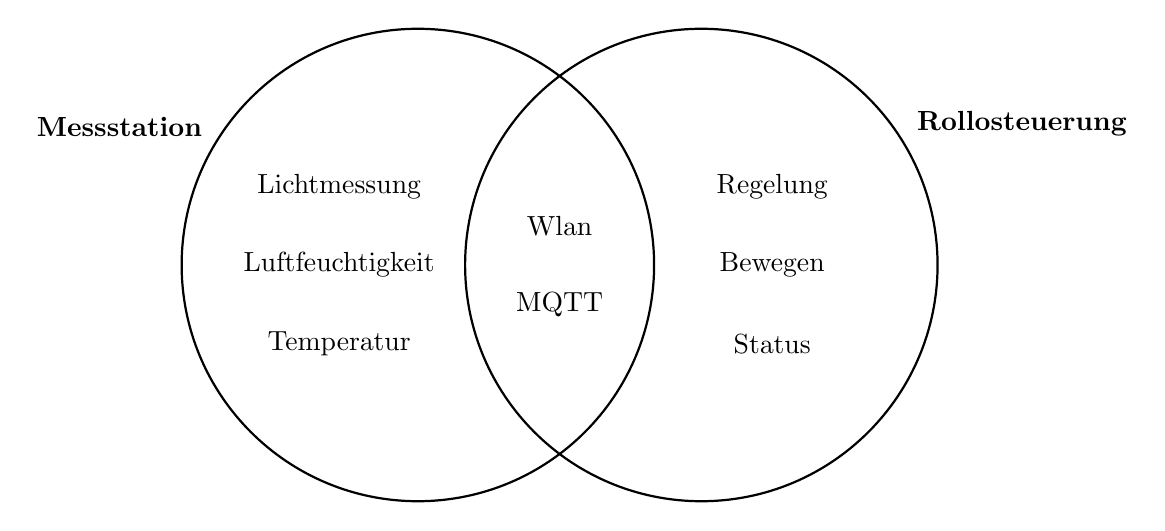
\begin{tikzpicture}[thick,
        set/.style = {circle,
            minimum size = 6cm,
        }]
     
        % Set A
        \node[set,label={150:\textbf{Messstation}}] (A) at (0,0) {};
        
        % Set B
        \node[set,label={30:\textbf{Rollosteuerung}}] (B) at (3.6,0) {};
        
        % Intersection
        \begin{scope}
            \clip (0,0) circle(3cm);
            \clip (3.6,0) circle(3cm);
        \end{scope}
        
        % Circles outline
        \draw (0,0) circle(3cm);
        \draw (3.6,0) circle(3cm);
        
        % Set intersection label
        \node at (1.8,0.5) {Wlan};
        \node at (1.8,-0.5) {MQTT};
        
        \node at (-1,1) {Lichtmessung};
        \node at (-1,0) {Luftfeuchtigkeit};
        \node at (-1,-1) {Temperatur};

        \node at (4.5,1) {Regelung};
        \node at (4.5,0) {Bewegen};
        \node at (4.5,-1) {Status};
     
    \end{tikzpicture}
    \caption{Darstellung der Verteilung von Funktionen der beiden Mikrocontroller}\label{fig:funk_schnitt}
\end{figure}

\section{Ablaufdiagramm}
\begin{figure}[H]
    \centering
    \begin{tikzpicture}[thick,scale=1, every node/.style={scale=1}]
        \node[activity] (callback){Nachricht};

        \node[decision,right = of callback] (decision1) {Funktion};

        \node[activity,above right  = 0.25cm  and 2cm   of decision1] (action1) {manuell()};
        \node[activity,above        = 0.7cm             of action1] (action2) {messung()};
        \node[activity,below right  = 0.25cm  and 2cm   of decision1] (action3) {automatik()};
        \node[activity,below        = 0.7cm             of action3] (action4) {Modus ändern};

        \node[end,below right       = 0.7cm   and 1cm   of action1](end){};

        \path [arrow line] (callback) -- (decision1);
        \path [arrow line] (decision1) |- node [above, near end]{steuerung}(action1);
        \path [arrow line] (decision1) |- node [above, near end]{status}(action2);
        \path [arrow line] (decision1) |- node [below, near end]{licht}(action3);
        \path [arrow line] (decision1) |- node [below, near end]{modus}(action4);

        \path [arrow line] (action1) -| (end);
        \path [arrow line] (action2) -| (end);
        \path [arrow line] (action3) -| (end);
        \path [arrow line] (action4) -| (end);
    \end{tikzpicture} 
    \caption{Ablaufdiagramm der Callback-Funktion}\label{fig:rollo_callback}
\end{figure}





\chapter{Fazit}
Innerhalb des Projektes wurden sieben Arbeitspakete definiert und nach der entsprechenden 
Reihenfolge bearbeitet. Aufgrund von einem internen Systemausfall konnten nicht alle dieser 
Arbeitspakete während der Durchführung dieses Projektes abgeschlossen werden. 
Abgeschlossen wurde eine intensive Einarbeitung in die Programmiersprache Python, die 
internen Systeme, eine Ist-Analyse und die Entwicklung eines theoretischen Modells. 
Die Implementierung der Funktion, das Testen und die Dokumentation konnten aufgrund der 
Systemstörung nicht abgeschlossen werden. 

Diese Praxisphase legt dennoch den Grundstein für die weitere Entwicklung und Implementierung
einer Funktion zur Erkennung von Grenzwertüberschreitungen der Temperatur bei rotierenden 
Maschinen. Des Weiteren wurden die zentralen Themen \glqq Agile Softwareentwicklung\grqq{} und 
\glqq Modulare, containerisierte Softwareapplikationen\grqq{} theoretisch erarbeitet und damit 
eine Vorbereitung für die Bearbeitung der Bachelorthesis  \glqq Entwicklung eines 
Prototyp-Algorithmus zur Ermittlung des Schmierzustandes eines Kugellagers an rotierenden 
Maschinen\grqq{} geschaffen. 





%===============================================================================

\pagenumbering{Roman}
%Literaturverzeichnis
\addcontentsline{toc}{chapter}{Literaturverzeichnis}\printbibliography[title=Literaturverzeichnis]
%Anhang
\appendix
\let\stdsection\section
\renewcommand\section{\newpage\stdsection}
\renewcommand{\thesection}{\Alph{section}}
\renewcommand*{\sectionmark}[1]{\markright{\MakeMarkcase{Anhang \thesection: #1}}}
\addcontentsline{toc}{chapter}{Anhang}

\includepdf[pages=-,scale = 0.8,
  pagecommand={},
  addtotoc={1,section,1,{Lastdrehmomentkurve},{app:lastdrehmoment}}
]{sections/appendix/lastdrehmoment.pdf}

\lstset{
    captionpos=top,
    language=C++,
    backgroundcolor=\color{white}
}

%Verbindung
\section{Quellcode MQTT und WiFi Verbindung}\label{sec:bib_mqtt_wlan}

\subsection{Header der Connection Library}
\lstinputlisting[label={lst:con_header},caption = ConnectionWiFi.h]{sections/appendix/ConnectionWifi/ConnectionWiFi.h}



\end{document}
